%   % !TEX root = ../../VIII,3_Rahmen-TeX_8-1.tex
%
%
%   Band VIII, 3 N.~??Z.2 (ex: ??A28)
%   Signatur/Tex-Datei: LH_35_10_08_010-011
%   RK-Nr. 60064
%   Überschrift: De vi elastica ad rationes geometricas revocata tentamen
%   Modul: Mechanik / AEF (Elastizität)
%   Datierung: 27 August 1689 (Verweis auf Juli 1686)
%   WZ: keins
%   SZ: keins
%   Bilddateien (PDF): LH_35_10_08_010-011_d1; LH_35_10_08_010-011_d2; LH_35_10_08_010-011_d3 (insgesamt: drei)
%   e Storckio
%
%
\selectlanguage{ngerman}%
\frenchspacing%
%
\begin{ledgroupsized}[r]{120mm}
\footnotesize
\pstart
\noindent\textbf{Überlieferung:}
\pend
\end{ledgroupsized}
\begin{ledgroupsized}[r]{114mm}
\footnotesize
\pstart \parindent -6mm
\makebox[6mm][l]{\textit{L}}%
Konzept: LH~XXXV~10,~8 Bl.~10\textendash11.
Ein Bogen 2\textsuperscript{o};
Einriss im Falz mit geringfügigem Textverlust am unteren Rand von Bl.~10~r\textsuperscript{o}.
Vier Seiten.
Auf Bl.~10~r\textsuperscript{o} am linken Rand, von Leibnizens Hand: $y=a^x$ \!\lbrack/\rbrack\ $ly=xla$;
am oberen Rand, ebenfalls von Leibnizens Hand quer:
$\ 4\ \ \frac{1}{4}\ \ \lbrack/\rbrack\ \ 3\ \ \frac{1}{3}\ \ \lbrack/\rbrack\ \ 2\ \ \frac{1}{2}\ .$
% N.~??Z.2/A28 hängt inhaltlich mit N.~??Z.1/A29 zusammen.
\pend
\end{ledgroupsized}
%
% \vspace*{5mm}
% \begin{ledgroup}
% \footnotesize
% \pstart
% \noindent\textbf{Datierungsgründe:}
% Es ist nicht eindeutig, ob Leibnizens eigenhändige Datierung sich auf die Abfassung des Textes oder auf seine Randbemerkungen bezieht. ???
% \pend
% \end{ledgroup}
%
\selectlanguage{latin}%
\frenchspacing%
%
%
\vspace{7mm}%
\count\Bfootins=900
\count\Afootins=900
\count\Cfootins=900
\pstart%
\noindent%
\normalsize%
\edtext{}{%
\lemma{\textit{Unter dem Datum:}}\Afootnote{%
(\protect\vphantom)%
Haec accurate constituta Jul. 1686.%
\protect\vphantom()\textsuperscript{\lbrack a\rbrack}% \\%
\vspace{0.3em}%
\newline%
{\footnotesize%
\textsuperscript{\lbrack a\rbrack}
(\protect\vphantom)%
Haec \lbrack...\rbrack\ 1686.%
\protect\vphantom()
Siehe N.~27\textsubscript{1}.\vspace{-4mm}}}}%
%
\edtext{\lbrack10~r\textsuperscript{o}\rbrack\ %%%%    Blatt 10r
%
27 Aug. 1689%
%
}{%
\lemma{\lbrack10~r\textsuperscript{o}\rbrack}\Bfootnote{%
\textit{(1)}~26
\textit{(2)}~27%
~\textit{L}}}%
\label{LH_35_10_08_010r_Marg_1686}
\pend%
\vspace{0.4em}%
%
\pstart\noindent
\centerline{%
De vi Elastica\protect\index{Sachverzeichnis}{vis elastica}
ad rationes Geometricas\protect\index{Sachverzeichnis}{ratio geometrica}
revocata Tentamen.\protect\index{Sachverzeichnis}{tentamen}}%
\pend%
\vspace{0.4em}%
%
%
\pstart%
\noindent%
Ponamus\edlabel{LH_35_10_08_010-011_ersterTeil-1}
%
\edtext{vasi\protect\index{Sachverzeichnis}{vas aere plenum} \textit{ABCD}}{%
\lemma{vasi \textit{ABCD}}\Cfootnote{%
Siehe das Diagramm \lbrack\textit{Fig.~1}\rbrack\ auf S.~\pageref{LH_35_10_08_010r_Fig.1}.}}
%
cujus latera \textit{AB}, \textit{DC} horizonti parallela inclusum esse aerem,\protect\index{Sachverzeichnis}{aer inclusus}
\edtext{et operculo\protect\index{Sachverzeichnis}{operculum mobile}}{%
\lemma{et}\Bfootnote{%
\textit{(1)}~operculum
\textit{(2)}~operculo%
~\textit{L}}}
%
\textit{EF} vas\protect\index{Sachverzeichnis}{vas aere plenum} exacte claudi,
ita tamen ut operculum\protect\index{Sachverzeichnis}{operculum mobile} sit
\edtext{mobile faciatque}{%
\lemma{mobile}\Bfootnote{%
\textit{(1)}~, eoque
\textit{(2)}~faciatque%
~\textit{L}}}
%
officium emboli,\protect\index{Sachverzeichnis}{embolus}
atque vi externa\protect\index{Sachverzeichnis}{vis externa}
ad comprimendum aerem\protect\index{Sachverzeichnis}{aer compressus}
in vas\protect\index{Sachverzeichnis}{vas aere plenum} intrudi possit.
% \pend%
%
%
% \pstart%
Esto
\edtext{jam globus\protect\index{Sachverzeichnis}{globus incurrens} \textit{H}
determinati ponderis,\protect\index{Sachverzeichnis}{pondus corporis impingentis}
qui}{%
\lemma{jam}\Bfootnote{%
\textit{(1)}~corpus
\textit{(2)}~globus \textit{H} determinati ponderis,
\textit{(a)}~quod
\textit{(b)}~qui%%
~\textit{L}}}
%
certa velocitate\protect\index{Sachverzeichnis}{velocitas compressionis}
veniens in linea horizonti parallela \textit{{\scriptsize0}H{\scriptsize1}H}
directe incurrat in embolum,\protect\index{Sachverzeichnis}{embolus}
eumque adigat in
\edtext{vas\protect\index{Sachverzeichnis}{vas aere plenum}
ab \textit{{\scriptsize1}E{\scriptsize1}F} ad \textit{{\scriptsize2}E{\scriptsize2}F}}{%
\lemma{vas}\Bfootnote{%
\textit{(1)}~ubicunque
\textit{(2)}~ab \textit{{\scriptsize1}E{\scriptsize1}F} ad \textit{{\scriptsize2}E{\scriptsize2}F}%
~\textit{L}}}
%
atque ita aerem comprimat%
\edtext{, ex spatio \textit{{\scriptsize1}E{\scriptsize1}FCB}\protect\index{Sachverzeichnis}{spatium compressionis}
in spatium \textit{{\scriptsize2}E{\scriptsize2}FCB}.}{%
\lemma{\hspace{-1,0mm}, ex}\Bfootnote{%
\hspace{-0,5mm}spatio \lbrack...\rbrack\ spatium \textit{{\scriptsize2}E{\scriptsize2}FCB} % \textit{{\scriptsize1}E{\scriptsize1}FCB} in
\textit{erg.~L}}} 
\pend%
%
%
%\count\Bfootins=1100
%\count\Afootins=1100
%\count\Cfootins=1100
\pstart%
Certum est corpus\protect\index{Sachverzeichnis}{corpus comprimens}
tantum suae potentiae\protect\index{Sachverzeichnis}{potentia amissa} amisisse
quanta est potentia quam tribuit aeri compresso.\protect\index{Sachverzeichnis}{aer compressus}
Ponamus ergo corpus continuando impetum,\protect\index{Sachverzeichnis}{impetus corporis incurrentis}
licet paulatim debilitatum
\edtext{adigere Embolum \textit{{\scriptsize1}E{\scriptsize1}F} primum in}{%
\lemma{adigere}\Bfootnote{%
\textit{(1)}~embolum primum in
\textit{(2)}~Embolum \textit{{\scriptsize1}E{\scriptsize1}F} primum in%
~\textit{L}}}
%
\textit{{\scriptsize2}E{\scriptsize2}F} ut dixi,
deinde in \textit{{\scriptsize3}E{\scriptsize3}F},
ac denique in \textit{{\scriptsize4}E{\scriptsize4}F},
atque ibi omni vi\protect\index{Sachverzeichnis}{vis consumta} sua consumta quiescere,
nec embolum\protect\index{Sachverzeichnis}{embolus} profundius
in vas\protect\index{Sachverzeichnis}{vas aere plenum} intrudere posse.
Vis\protect\index{Sachverzeichnis}{vis aeris elastica} ergo
Elastri aeris\protect\index{Sachverzeichnis}{elastrum aeris}
\edtext{cujus spatium\protect\index{Sachverzeichnis}{spatium naturale} naturale}{%
\lemma{cujus}\Bfootnote{%
\textit{(1)}~status naturalis
\textit{(2)}~spatium naturale%
~\textit{L}}}
%
erat \textit{{\scriptsize1}E{\scriptsize1}FCB},
compressi\protect\index{Sachverzeichnis}{aer compressus}
intra spatium\protect\index{Sachverzeichnis}{spatium compressionis}
%%%%%%%%%%%%%%%%%%%%%%%%%%%%%%%%%%%%%%%%%%%%%%%%%%%%%%%%%Künstlicher Seitenumbruch mit LabelfootnoteKZEitz
\edlabel{KZeitz3}%
\makebox[1.0\textwidth][s]{\textit{{\scriptsize4}E{\scriptsize4}FCB} aequabitur potentiae corporis \textit{H}
quam habebat cum initio impingeret, in \textit{{\scriptsize0}H}}%
\edtext{}%
{{\xxref{KZeitz3}{KZeitz4}}%
{\lemma{\textit{{\scriptsize4}E{\scriptsize4}FCB}}\Bfootnote{\textit{(1)}~metietur
\textit{(2)}~mensurari etiam poteri
\textit{(3)}~aequabitur
\textit{(4)}~aequabitur potentiae corporis \textit{H}
\textit{(a)}~initio
\textit{(b)}~quam habebat cum initio impingeret,
\textbar~hoc est \textit{gestr.}~%
\textbar\ in \textit{{\scriptsize0}H} seu \textit{{\scriptsize1}H},
\textit{(aa)}~nempe
\textit{(bb)}~et mensurabitur per%
~\textit{L}}}}%
\pend
\newpage
\pstart
\noindent 
%%%%%%%%%%%%%%%%%%%%%%%%%%%%%%%%%%%%%%%%%%%%%%%%%%%%%%%%%%%%%%%%%%%%%%%%%%%%%%%%%
seu \textit{{\scriptsize1}H},
et mensurabitur per\edlabel{KZeitz4} factum ex magnitudine corporis \textit{H},\protect\index{Sachverzeichnis}{magnitudo corporis}
ducta in quadratum celeritatis,\protect\index{Sachverzeichnis}{quadratum celeritatis}
qua impingebat.\protect\index{Sachverzeichnis}{velocitas corporis impingentis}
\edtext{Et vicissim velocitas corporis\protect\index{Sachverzeichnis}{velocitas corporis impingentis}
haberi poterit per Elastrum\protect\index{Sachverzeichnis}{elastrum aeris} aeris
quod effecit.}{%
\lemma{Et}\Bfootnote{\hspace{-0,5mm}%
vicissim \lbrack...\rbrack\ per Elastrum % velocitas corporis haberi poterit
\textit{(1)}~aeris
\textit{(2)}~aeris quod effecit.
\textit{erg.~L}}}
\pend%
\pstart%
Porro potentiae ejusdem aeris\protect\index{Sachverzeichnis}{potentia aeris compressi}
plus minusve compressi sunt inter se,
in reciproca ratione spatiorum\protect\index{Sachverzeichnis}{spatium compressionis}
in quibus continentur.
Et
\edtext{quidem potentia aeris}{%
\lemma{quidem}\Bfootnote{%
\textit{(1)}~quam aer
\textit{(2)}~potentia aeris%
~\textit{L}}}
%
Elastica\protect\index{Sachverzeichnis}{potentia aeris elastica}
in statu\protect\index{Sachverzeichnis}{status naturalis} natu-
\pend
\vspace{1.5em}
  \centerline{\hspace*{10mm}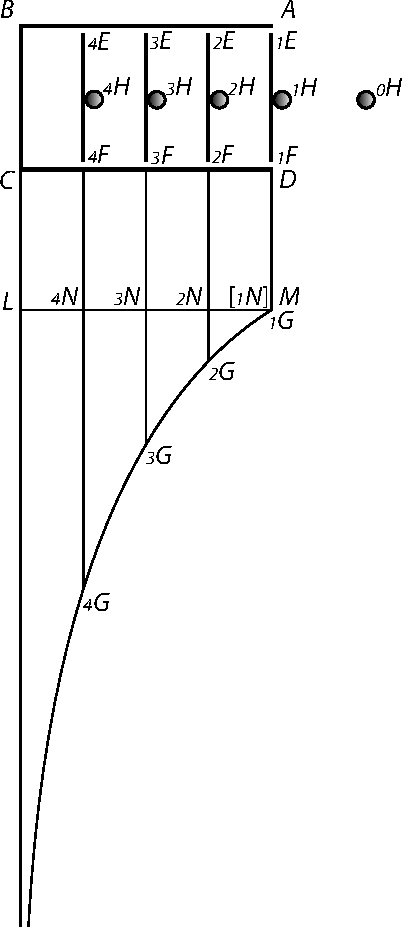
\includegraphics[width=0.40\textwidth]{gesamttex/edit_VIII,3/images/LH_35_10_08_010-011_d1.pdf}}%
  \vspace{-1.5em}
  \centerline{\hspace*{10mm}\lbrack\textit{Fig.~1}\rbrack}%
  \label{LH_35_10_08_010r_Fig.1}%
  \newpage
  \count\Bfootins=1100
\count\Afootins=1100
\count\Cfootins=1100
\pstart
\noindent
rali, si cogitatione\protect\index{Sachverzeichnis}{cogitatio} auferatur
pondus aeris incumbentis,\protect\index{Sachverzeichnis}{pondus aeris}
est tanta quanta est ipsum pondus aeris incumbentis,
quod\protect\index{Sachverzeichnis}{pondus aeris}
\edtext{repraesentemus per \textit{DM} vel per \textit{{\scriptsize1}F{\scriptsize1}G};
potentiam\protect\index{Sachverzeichnis}{potentia aeris compressi}}{%
\lemma{repraesentemus}\Bfootnote{%
\textit{(1)}~per \textit{D{\scriptsize1}G}
\textit{(2)}~per \textit{DM} vel per \textit{{\scriptsize1}F{\scriptsize1}G}
\textit{(a)}~vel \textit{D}
\textit{(b)}~; potentiam%
~\textit{L}}}
%
aeris compressi in \textit{{\scriptsize2}E{\scriptsize2}FBC}
exprimamus per \textit{{\scriptsize2}F{\scriptsize2}G},
compressi in \textit{{\scriptsize3}E{\scriptsize3}FBC}
repraesentemus per \textit{{\scriptsize3}F{\scriptsize3}G}
et ita porro;
\edlabel{LH_35_10_08_010r_umgekehrtProp_casdg-1}%
ita ut semper sit
\edtext{\textit{FG} ad \textit{DM}}{%
\lemma{\textit{FG}}\Bfootnote{%
\hspace{-0,5mm}ad
\textit{(1)}~\textit{DC}
\textit{(2)}~\textit{DM}%
~\textit{L}}}
%
ut \textit{CD} ad \textit{CF}, seu
\edtext{sint ipsae \textit{FG}}{%
\lemma{sint}\Bfootnote{%
\textit{(1)}~\textit{FG}
\textit{(2) }ipsae \textit{FG}%
~\textit{L}}}
%
ipsis \textit{CF} reciproce proportionales,
verbi
\edtext{gratia \textit{{\scriptsize2}F{\scriptsize2}G} ad \textit{{\scriptsize1}F{\scriptsize1}G} ut}{%
\lemma{gratia}\Bfootnote{%
\textit{(1)}~\textit{C{\scriptsize2}F} ad \textit{{\scriptsize1}F{\scriptsize1}C} ut
\textit{(2)}~\textit{{\scriptsize2}F{\scriptsize2}G} ad \textit{{\scriptsize1}F{\scriptsize1}G} ut%
~\textit{L}}}
%
\textit{C{\scriptsize1}F} ad \textit{C{\scriptsize2}F};%
\edlabel{LH_35_10_08_010r_umgekehrtProp_casdg-2}
erit
\edtext{\lbrack ergo\rbrack}{%
\lemma{ergo}\Bfootnote{%
\textit{erg. Hrsg.}}}
%
linea \textit{GG} Hyperbola,\protect\index{Sachverzeichnis}{hyperbola}
cujus centrum \textit{C},
asymptota una \textit{CD},
altera \textit{BC} vel \textit{CL}.
\pend%
%
%
\pstart%
\edtext{}{%
{\xxref{LH_35_10_08_010r_suurihuomaus-1}{LH_35_10_08_010r_suurihuomaus-2}}%
{\lemma{\textit{Am Rand:}}\Afootnote{%
Videtur error\protect\index{Sachverzeichnis}{error} subesse,
compressiones\protect\index{Sachverzeichnis}{compressio aeris} quidem
sunt reciproce proportionales spatiis,\protect\index{Sachverzeichnis}{spatium compressionis}
adeoque et vires\protect\index{Sachverzeichnis}{vis compressionis}
quae in ea compressione tenere possunt.
Sed aliae sunt vires quae in ea compressione tenere possunt,
aliae vero sunt vires jam assumtae ad producendam % \textsuperscript{\lbrack a\rbrack}
illam compressionem,\protect\index{Sachverzeichnis}{vis comprimens}
seu quae tot\textlangle a\textrangle\ illa restitutione\protect\index{Sachverzeichnis}{restitutio aeris} possunt recuperari.\textsuperscript{\lbrack a\rbrack}
Et dubium est finiri compressionem,\protect\index{Sachverzeichnis}{compressio aeris}
quando vis globi impingentis\protect\index{Sachverzeichnis}{globus impingens}
exhausta,\protect\index{Sachverzeichnis}{vis exhausta}
videtur enim finiri,
quando illa vis ei adhuc residua in aequilibrio\protect\index{Sachverzeichnis}{aequilibrium} est
cum ipsa vi \lbrack compressioni\rbrack\textsuperscript{\lbrack b\rbrack} resistente.\protect\index{Sachverzeichnis}{vis resistens}
\newline
\hspace*{7,5mm}%
Jam videtur id rectum esse,
nam non apparet,
ubi vis ejus sit\protect\index{Sachverzeichnis}{vis corporis comprimentis}
cum utique quiescat,
nisi translata\protect\index{Sachverzeichnis}{vis translata} sit tota
in aerem comprimendum,\protect\index{Sachverzeichnis}{aer comprimendus}
posito compressionem nullam esse in ipso corpore \textit{H}\textsuperscript{\lbrack c\rbrack},
quod fingimus rigidissimum.\protect\index{Sachverzeichnis}{corpus rigidissimum}
\newline
\hspace*{7,5mm}%
NB: Videndum an non dicendum sit potius
ipsas \textit{NG} non esse ut vires totas,\protect\index{Sachverzeichnis}{vis compressionis}
sed ut crementa,
spatia vero seu summas eorum esse ut vires totas,
ita ut corpus \textit{H} impetu suo comprimens%
\protect\index{Sachverzeichnis}{corpus comprimens}\protect\index{Sachverzeichnis}{impetus corporis comprimentis}
in \textit{{\scriptsize2}H} perdat vim
ut \textit{{\scriptsize2}N{\scriptsize2}G}.
Et ita esse video ponendo infinita
quasi Elastra inaequalia,\protect\index{Sachverzeichnis}{elastrum inaequale}
in ratione compressionum,\protect\index{Sachverzeichnis}{compressio aeris}
sed tendenda per aequale spatium infinite parvum impetu illapsus.
Ergo totae vires amissae\protect\index{Sachverzeichnis}{vis amissa}
\textlangle su\textrangle nt ut spatia\protect\index{Sachverzeichnis}{spatium compressionis}
seu ut logarithmi\protect\index{Sachverzeichnis}{logarithmus}
et celeritates ut radices logarithmorum.\protect\index{Sachverzeichnis}{radix quadratica logarithmi}% \\%
\vspace{0.5em}%
\newline%
{\footnotesize %
% \textsuperscript{\lbrack a\rbrack} assumtae
% \textit{(1)}~ad pr
% \textit{(2)}~ad producendam%
% ~\textit{L}\hspace{5mm}
\textsuperscript{\lbrack a\rbrack}~%
recuperari.~%
\textit{(1)}~Nec
\textit{(2)}~Et
\textit{(a)}~falsum
\textit{(b)}~dubium%
~\textit{L}
\quad%
\textsuperscript{\lbrack b\rbrack}~%
compressionis \textit{L~ändert Hrsg.}%
\quad%
\textsuperscript{\lbrack c\rbrack}~%
\textit{H} \textit{erg.~L}\vspace{-3mm}}}}}%
%
%
Cum\edlabel{LH_35_10_08_010r_suurihuomaus-1}\edlabel{LH_35_10_08_010r_utsupra_bguzbfiv-1}
ergo potentia\protect\index{Sachverzeichnis}{potentia corporis comprimentis}
\edtext{corporis \textit{H} durante emboli\protect\index{Sachverzeichnis}{embolus} intrusione
jam amissa\protect\index{Sachverzeichnis}{potentia amissa} praecise tanta sit,}{%
\lemma{corporis \textit{H}\hspace{-0,5mm}}\Bfootnote{%
\textit{(1)}~existentis in puncto aliquo
\textit{(2)}~durante emboli intrusione
\textit{(a)}~quam amissa, praeci
\textit{(b)}~adhuc residua praecise tanta sit
\textit{(c)}~jam amissa praecise tanta sit,%
~\textit{L}}}
%
quanta est vis\protect\index{Sachverzeichnis}{vis aeris elastica}
Elastri aerei\protect\index{Sachverzeichnis}{elastrum aereum} in illo loco,
erit
%
%
\edtext{}{{\xxref{KZeitz127}{KZeitz128}}%
{%
\lemma{ergo}\Bfootnote{\hspace{-0,5mm}%
\textbar~et in \lbrack...\rbrack\ rursus exploditur, \textit{erg.}~% restitutione, qua corpus \textit{H} 
\textbar\ vis
\textit{(1)}~Emboli in
\textit{(2)}~corporis \textit{H} in%
~\textit{L}}}}
\edlabel{KZeitz127}ergo et in restitutione,\protect\index{Sachverzeichnis}{restitutio aeris}
qua corpus \textit{H} rur-
\pend
\newpage
\pstart
\noindent sus exploditur,\protect\index{Sachverzeichnis}{corpus explosum}
\edlabel{LH_35_10_08_010r_falschepropror_adfg-1}vis corporis \textit{H} in\edlabel{KZeitz128}
%
\edtext{}{%
{\xxref{LH_35_10_08_010r_falschepropror_adfg-1}{LH_35_10_08_010r_falschepropror_adfg-2}}%
{\lemma{vis corporis \lbrack...\rbrack\ ad \textit{DM}}\Cfootnote{%
In \textit{{\scriptsize{2}}H} und \textit{{\scriptsize{1}}H} kommt dem Körper \textit{H} jeweils eine Bewegungskraft zu,
die vielmehr in \textit{umgekehrtem} Verhältnis zu den Größen \textit{{\scriptsize{2}}F{\scriptsize{2}}G} und \textit{{\scriptsize{1}}F{\scriptsize{1}}G} (bzw. \textit{DM}) stehen.
Vgl. S.~\refpassage{LH_35_10_08_010r_umgekehrtProp_casdg-1}{LH_35_10_08_010r_umgekehrtProp_casdg-2}.}}}%
\textit{{\scriptsize2}H} ad vim corporis \textit{H}\protect\index{Sachverzeichnis}{vis corporis comprimentis}
in \textit{{\scriptsize1}H}, ut \textit{{\scriptsize2}F{\scriptsize2}G} ad \textit{{\scriptsize1}F{\scriptsize1}G} seu ad \textit{DM},%
\edlabel{LH_35_10_08_010r_falschepropror_adfg-2}\edlabel{LH_35_10_08_010r_utsupra_bguzbfiv-2}
si
\edtext{scilicet pondus\protect\index{Sachverzeichnis}{pondus aeris}
\lbrack aeris\rbrack\ externi\protect\index{Sachverzeichnis}{aer externus} amotum,
ac res in vacuo\protect\index{Sachverzeichnis}{vacuum} acta intelligatur,}{%
\lemma{scilicet}\Bfootnote{%
\textit{(1)}~ponas
\textit{(2)}~pondus \textbar~aeri \textit{ändert Hrsg.}~\textbar\ externi amotum, \lbrack...\rbrack\ acta intelligatur,%
~\textit{L}}}
%
obice\protect\index{Sachverzeichnis}{obex} forte opposito
ne aer\protect\index{Sachverzeichnis}{aer inclusus}
\edtext{inclusus in \textit{{\scriptsize1}E{\scriptsize1}FCB}}{%
\lemma{inclusus}\Bfootnote{%
\hspace{-0,5mm}in
\textit{(1)}~\textit{{\scriptsize1}F{\scriptsize1}G}
\textit{(2)}~\textit{{\scriptsize1}E{\scriptsize1}FCB}%
~\textit{L}}}
%
embolum\protect\index{Sachverzeichnis}{embolus} plane extrudat. 
\pend%
 \count\Bfootins=1100
\count\Afootins=1100
\count\Cfootins=1100
%
%
\pstart%
Sed in aere libero\protect\index{Sachverzeichnis}{aer liber}
\edtext{ubique}{%
\lemma{ubique}\Bfootnote{%
\textit{erg.~L}}}
%
detrahenda est vis aeris incumbentis%
\protect\index{Sachverzeichnis}{vis aeris incumbentis}\protect\index{Sachverzeichnis}{aer incumbens}
repraesentata per \textit{DM},
ducatur ergo recta \textit{ML} parallela ipsi \textit{CD},
seu normalis ad \textit{BCL}, secans ipsas \textit{FG} in punctis \textit{N}.
Et vires Elastri aerei\protect\index{Sachverzeichnis}{vis aeris elastica}\protect\index{Sachverzeichnis}{elastrum aereum}
in quolibet compressionis statu\protect\index{Sachverzeichnis}{status compressionis}
repraesentabuntur per rectas \textit{NG},
exempl. gr. in \textit{{\scriptsize1}E{\scriptsize1}F} statu naturali,\protect\index{Sachverzeichnis}{status naturalis}
potentia\protect\index{Sachverzeichnis}{potentia compressionis} haec erit nulla,
quia et nulla compressio;\protect\index{Sachverzeichnis}{compressio aeris}
in statu \textit{{\scriptsize2}E{\scriptsize2}FCB}\protect\index{Sachverzeichnis}{status compressionis}
repraesentabitur per \textit{{\scriptsize2}N{\scriptsize2}G},
seu
\edtext{erit ad vim aeris incumbentis\protect\index{Sachverzeichnis}{vis aeris incumbentis}
(\protect\vphantom)quae determinata habetur
aliunde%
% \edtext{}{%
% \lemma{aliunde}\Cfootnote{ ??}}
% PR: Das ist keine konkrete Anspielung, sondern eine allgemeine: "Man weiß aus anderen Gründen, dass die Kraft der über uns schwebenden Luft bestimmt ist. 
\protect\vphantom() ut \textit{{\scriptsize2}N{\scriptsize2}G} ad \textit{DM}.}{%
\lemma{erit}\Bfootnote{%
\textit{(1)}~ad \textit{DM},
\textit{(2)}~ad vim \lbrack...\rbrack\ ad \textit{DM}.%
~\textit{L}}}
%
Et ita \edlabel{LH_35_10_08_010-011_e010r1}porro.
% \edtext{}{%
% {\xxref{LH_35_10_08_010-011_e010r1}{LH_35_10_08_010-011_e010r2}}%
% \lemma{porro.}\Bfootnote{%
% \textit{(1)}~Vis ergo corporis
% \textit{(2)}~Vis ergo corporis%
% ~\textit{L}}}
\pend%
%
%
\pstart%
Vis\protect\index{Sachverzeichnis}{vis corporis comprimentis}
ergo corporis\edlabel{LH_35_10_08_010-011_e010r2}
\textit{H}\protect\index{Sachverzeichnis}{corpus comprimens} tota
quam initio in \textit{{\scriptsize0}H} vel \textit{{\scriptsize1}H} habuit,
repraesentabitur per ultimam \textit{{\scriptsize4}N{\scriptsize4}G},
seu erit ad vim\protect\index{Sachverzeichnis}{vis aeris elastica}
quam
\edtext{aeris Elastrum naturale\protect\index{Sachverzeichnis}{elastrum aeris naturale} apud}{%
\lemma{aeris}\Bfootnote{%
\textit{(1)}~in statu
\textit{(2)}~apu
\textit{(3)}~Elastrum naturale apud%
~\textit{L}}}
%
nos habet,
ut \textit{{\scriptsize4}N{\scriptsize4}G} ad
%
\edtext{\lbrack\textit{DM}\rbrack,}{%
\lemma{\textit{DG}}\Bfootnote{%
\textit{L~ändert Hrsg.}}}
%
quia scilicet ultima \textit{{\scriptsize4}N{\scriptsize4}G}
\edtext{exprimit vim Elasticam aeris,\protect\index{Sachverzeichnis}{vis aeris elastica}}{%
\lemma{exprimit}\Bfootnote{%
\textit{(1)}~Elastrum aeris maxi
\textit{(2)}~vim Elasticam aeris,%
~\textit{L}}}
%
quam tota vi corporis \textit{H} exhausta\protect\index{Sachverzeichnis}{vis exhausta} accepit,
quae proinde ipsi vi corporis\protect\index{Sachverzeichnis}{vis corporis comprimentis}
quam initio integram\protect\index{Sachverzeichnis}{vis integra} habuit,
aequalis est,
quia ipsam
\edtext{totam aeri}{%
\lemma{totam}\Bfootnote{%
\textit{(1) }corpori 
\textit{(2)}~aeri%
~\textit{L}}}
%
compresso\protect\index{Sachverzeichnis}{aer compressus}
communicasse\protect\index{Sachverzeichnis}{vis communicata} suppono.\edlabel{LH_35_10_08_010r_suurihuomaus-2}
%
\lbrack 10~v\textsuperscript{o}\rbrack\ %%%% Blatt 10v
%
\pend%
%
\pstart%
Hinc jam facile est definire
quam corpus \textit{H}\protect\index{Sachverzeichnis}{corpus comprimens}
in quolibet loco residuam habeat celeritatem.\protect\index{Sachverzeichnis}{celeritas residua}
\edlabel{LH_35_10_08_010v_definitiones_usivc-1}%
Sit enim velocitas ejus prima \textit{v},\protect\index{Sachverzeichnis}{velocitas corporis comprimentis}
pondus autem ejus \textit{h},\protect\index{Sachverzeichnis}{pondus corporis comprimentis}
erit vis ejus prima \textit{hvv}.\protect\index{Sachverzeichnis}{vis corporis comprimentis}
Jam ponatur et nota vis\protect\index{Sachverzeichnis}{vis aeris elastica}
Elastri naturalis\protect\index{Sachverzeichnis}{elastrum aeris naturale}
%
\edtext{\lbrack aeris\rbrack;}{\lemma{aeris}\Bfootnote{\textit{erg. Hrsg.}}}
%
quae si ad idem corpus
\edtext{\lbrack \textit{H}\rbrack}{%
\lemma{\textit{h}}\Bfootnote{\textit{L~ändert Hrsg.}}}
esset
\edtext{accommodanda,
deberet corpus \textit{H}\protect\index{Sachverzeichnis}{corpus comprimens}
habere velocitatem \textit{e},\protect\index{Sachverzeichnis}{velocitas corporis comprimentis}}{%
\lemma{accommodanda,}\Bfootnote{%
\textit{(1)}~exprime
\textit{(2)}~deberet corpus
\textit{(a)}~fig
\textit{(b)}~\textit{H} habere velocitatem
\textit{(aa)}~\textit{ee}
\textit{(bb)}~\textit{4e}
\textit{(cc)}~\textit{e},%
~\textit{L}}}
%
itaque erit ea
\edtext{vis \textit{hee}}{%
\lemma{vis}\Bfootnote{%
\textit{(1)}~$\displaystyle h\overline{4e}^2$\!
\textit{(2)}~\textit{he}
\textit{(3)}~\textit{hee}%
~\textit{L}}}
%
eritque \textit{{\scriptsize4}N{\scriptsize4}G} ad
\edtext{\textit{DM} ut \textit{hvv} ad \textit{hee} seu ut \textit{vv} ad \textit{ee}.}{%
\lemma{\textit{DM}}\Bfootnote{%
\hspace{-0,5mm}ut
\textit{(1)}~\textit{e}
\textit{(2)}~$\displaystyle h\,\overline{4e}^2$ ad \textit{hvv} seu ut
\textit{(a)}~\textit{ee} ad \textit{vv}
\textit{(b)}~$\displaystyle\overline{4e}^2$\! ad \textit{v}
\textit{(3)}~\textit{hvv} ad \textit{hee} seu ut \textit{vv} ad \textit{ee}.%
~\textit{L}}}
%
Sit \textit{DM} aequ.
\edtext{\textit{m}
et \textit{C{\scriptsize4}F} seu \textit{L{\scriptsize4}N} aequ. \textit{t}%
\edlabel{LH_35_10_08_010v_definitiones_usivc-2}
et \textit{{\scriptsize4}N{\scriptsize4}G} vocemus $\theta.$
Fiet \textit{t}}{%
\lemma{\textit{m} et}\Bfootnote{%
\textit{(1)}~\textit{CF} aequ. \textit{f}
\textit{(2)}~\textbar~et \textit{streicht Hrsg.}~%
\textbar\ \textit{C{\scriptsize4}F}
\textbar~seu \textit{L{\scriptsize4}N} \textit{erg.}~%
\textbar\ aequ.
\textit{(a)}~\textit{G}
\textit{(b)}~\textit{v}
\textit{(c)}~\textit{t}
\textit{(aa)}~(\protect\vphantom)tota enim
\textit{(aaa)}~vim
\textit{(bbb)}~vis ibi est\protect\vphantom() erit
\textit{(bb)}~et \textit{{\scriptsize4}N{\scriptsize4}G} vocemus $\theta.$ Fiet
\textit{(aaa)}~$t\theta$ ae
\textit{(bbb)}~\textit{t}%
~\textit{L}}}
%
in
%
\edtext{$\displaystyle\stackrel{\displaystyle m+\theta}{\overbrace{\lbrack{\scriptstyle\textit{4}}F{\scriptstyle\textit{4}}G\rbrack}}$}{%
\lemma{\textit{{\scriptsize4}N{\scriptsize4}G}}\Bfootnote{%
\textit{L~ändert Hrsg.}}}
%
aequ. \textit{CD}\rule[-1,5mm]{0pt}{0mm}
\edtext{in \textit{DM} seu \textit{mm} si ponamus}{%
\lemma{in \textit{DM}}\Bfootnote{%
\textit{(1)}~ponamus
\textit{(2)}~seu
\textbar~in \textit{streicht Hrsg.}~%
\textbar\ \textit{mm} si ponamus%
~\textit{L}}}
%
\textit{CD} et \textit{DM} esse aequales,
fiet:
\pend
\newpage
 \count\Bfootins=1000
\count\Afootins=1000
\count\Cfootins=1000
\pstart%
\noindent \textit{t} in $\theta +m$ aequ. \textit{mm},
seu $\theta + m$ aequ.\rule[-2mm]{0pt}{7mm}
$\displaystyle\frac{mm}{t}.$
Est autem $\theta$ ad \textit{m} ut \textit{vv} ad \textit{ee}.
Ergo rursus $\theta$ aequ. % \rule[-6mm]{0pt}{12mm}
$\displaystyle\frac{mvv}{ee}$ aequ. % \rule[-4mm]{0pt}{4mm}
$\displaystyle\frac{mm}{t}-m.$
Ergo $vv:ee$ aequ.
\edlabel{LH_35_10_08_010-011_e010v1}$\overline{m-t}:t.$%
\edtext{}{%
{\xxref{LH_35_10_08_010-011_e010v1}{LH_35_10_08_010-011_e010v2}}%
{\lemma{$\displaystyle\overline{m-t}:t.$}\Bfootnote{%
\textit{(1)}~Idem plane est
\textit{(a)}~, si
\textit{(b)}~calculus si non locum \textit{{\scriptsize4}F}, sed
\textbar~alium ut \textit{erg.}~%
\textbar\ \textit{{\scriptsize3}F} assumsissemus, erit enim
\textit{(aa)}~\textit{ee} celeritas
\textit{(bb)}~\textit{hee} vis quam corpus \textit{H} amisit seu in Elastrum\protect\index{Sachverzeichnis}{elastrum aeris} aeris transmisit, \textit{e} celeritas quam amisit. Itaque
\textit{(aaa)}~\textit{h}
\textit{(bbb)}~\textit{e}
\textit{(ccc)}~celeritas
\textit{(aaaa)}~prima cor
\textit{(bbbb)}~integra corporis \textit{H} incurrentis, est ad
\textit{(aaaaa)}~celer
\textit{(bbbbb)}~\textit{v} celeritatem integram quam idem corpus habere deberet si vim
\textit{(2)}~Itaque $m-t$ seu
\textit{(a)}~\textit{{\scriptsize4}N}
\textit{(b)}~\textit{M{\scriptsize4}F} spatium \lbrack...\rbrack\ quarum illa
\textbar~\textit{v} \textit{erg.}~%
\textbar\ est quam \lbrack...\rbrack\ corpus \textit{H}, si % habere deberet
\textit{(aa)}~vim
\textit{(bb)}~tota vis \lbrack...\rbrack\ esset translata, % Elastri naturalis aeris in ipsum
\textit{(aaa)}~ad
\textit{(bbb)}~haec est \lbrack...\rbrack\ \textit{{\scriptsize3}F}, nempe
\textit{(aaaa)}~spatium \textit{M{\scriptsize3}F} vocemus \textit{s}, quod nempe aeri ademtum est. Nam si
\textit{(bbbb)}~erit
\textbar~erit \textit{streicht Hrsg.}~\textbar~%
\textit{(aaaaa)}~\textit{s} sp
\textit{(bbbbb)}~\textit{s} seu \textit{M{\scriptsize3}F} \lbrack...\rbrack\ venisse amisit.
\textit{(aaaaa-a)}~Sunt ergo spatia percu
\textit{(bbbbb-b)}~Seu erit
\textit{(aaaaa-aa)}~$s : t$ aequ. \textit{vv}
\textit{(bbbbb-bb)}~$s : t$ aequ. \lbrack...\rbrack\ constans, erunt % $vv : cc$ seu \textit{s} aequ. $tvv : cc$ cumque \textit{tvv} sit
\textit{(aaaaa-aaa)}~spatia s
\textit{(bbbbb-bbb)}~spatia \textit{MF}
\textit{(aaaaa-aaaa)}~percursa a corpore
\textit{(bbbbb-bbbb)}~seu \textit{s} percursa \lbrack...\rbrack\ reciproca celeritatum
\textit{(aaaaa-aaaaa)}~seu
\textit{(bbbbb-bbbbb)}~. Nempe \textit{s} \lbrack...\rbrack\ ad \textit{cc}.% \textit{(s)} ut $tvv:cc$ ad $tvv:\textit{(c)(c)}$ seu ut \textit{(c)(c)}
~\textit{L}}}}
\pend%
%
%
\pstart%
Itaque\rule[-2mm]{0pt}{6mm}
\edtext{$m-t$ seu \textit{M{\scriptsize4}F}}{%
\lemma{$m-t$ seu \textit{M{\scriptsize4}F}}\Cfootnote{%
Die Buchstaben \textit{m} und \textit{t} bezeichnen jetzt nicht mehr bloße Strecken (nach den Setzungen auf S.~\refpassage{LH_35_10_08_010v_definitiones_usivc-1}{LH_35_10_08_010v_definitiones_usivc-2}),
sondern die entsprechenden Rechtecke aus den Abszissen und den Ordinaten der Hyperbel \textit{GG}.}}
%
spatium aeri\protect\index{Sachverzeichnis}{aer compressus}
compresso ademtum,\protect\index{Sachverzeichnis}{spatium ademtum}
est ad
%
\textit{t} seu \textit{CM} spatium totum,\protect\index{Sachverzeichnis}{spatium compressionis}
in duplicata ratione celeritatum \textit{v} ad \textit{e},
\edtext{quarum illa \textit{v}\protect\index{Sachverzeichnis}{celeritas corporis comprimentis} est
quam habere deberet corpus \textit{H},\protect\index{Sachverzeichnis}{corpus comprimens}
si tota vis\protect\index{Sachverzeichnis}{vis aeris elastica}
Elastri naturalis aeris\protect\index{Sachverzeichnis}{elastrum aeris naturale}
in ipsum esset translata,\protect\index{Sachverzeichnis}{vis translata}
haec est illa quam actu\protect\index{Sachverzeichnis}{actus}
ante impulsum emboli\protect\index{Sachverzeichnis}{embolus} habuit.}{%
\lemma{quarum \lbrack...\rbrack\ habuit}\Cfootnote{%
Die Bedeutung von \textit{v} und \textit{e} wird hier verwechselt.
Vgl. die Setzungen auf S.~\refpassage{LH_35_10_08_010v_definitiones_usivc-1}{LH_35_10_08_010v_definitiones_usivc-2}.}}
\pend%
%
%
\pstart%
Idem calculus\protect\index{Sachverzeichnis}{calculus} locum habet
et in alio spatii puncto ut in \textit{{\scriptsize3}F},
nempe erit \textit{s} seu \textit{M{\scriptsize3}F}
seu spatium aeri\protect\index{Sachverzeichnis}{aer compressus}
a corporis impulsu\protect\index{Sachverzeichnis}{impulsus corporis comprimentis} ademtum,
ad \textit{t} seu \textit{CM} spatium totum,\protect\index{Sachverzeichnis}{spatium compressionis}
in duplicata ratione celeritatis \textit{v},
quae qualis sit jam determinavimus,
ad celeritatem \textit{c}\protect\index{Sachverzeichnis}{celeritas corporis comprimentis}
quam corpus \textit{H}\protect\index{Sachverzeichnis}{corpus comprimens}
cum eo venisse
amisit.\protect\index{Sachverzeichnis}{celeritas amissa}
Seu erit $s : t$ aequ. $vv : cc.$
seu \textit{s} aequ. $tvv:cc$ cumque \textit{tvv} sit constans,
erunt spatia \textit{MF} seu \textit{s} percursa\protect\index{Sachverzeichnis}{spatium percursum}
a corpore \textit{H}\protect\index{Sachverzeichnis}{corpus comprimens}
dum embolum\protect\index{Sachverzeichnis}{embolus} intrudit,
seu amissa\protect\index{Sachverzeichnis}{spatium amissum}
ab aere compresso,\protect\index{Sachverzeichnis}{aer compressus}
in duplicata ratione reciproca celeritatum.
Nempe \textit{s} ad \textit{(s)} ut $tvv:cc$ ad $tvv:\textit{(c)(c)}$ seu ut \textit{(c)(c)} ad \textit{cc}.%
\edlabel{LH_35_10_08_010-011_e010v2}
\pend%
%
%
\pstart%
Hinc\edlabel{LH_35_10_08_010v_utsupra_jzfgik-1} jam facile colligitur
quam vim\protect\index{Sachverzeichnis}{vis aeris compressi}\protect\index{Sachverzeichnis}{vis aeris se restituentis}
aer compressus\protect\index{Sachverzeichnis}{aer compressus}
ac sese restituens\protect\index{Sachverzeichnis}{aer se restituens}
corpori projiciendo\protect\index{Sachverzeichnis}{corpus projiciendum}
communicet.\protect\index{Sachverzeichnis}{vis communicata}
Ponamus enim aerem compressum\protect\index{Sachverzeichnis}{aer compressus}
corpus \textit{H}\protect\index{Sachverzeichnis}{corpus comprimens}
quod vim\protect\index{Sachverzeichnis}{vis comprimendi}
%
\edtext{\lbrack comprimendi\rbrack}{\lemma{comprimendo}\Bfootnote{\textit{L~ändert Hrsg.}}}
%\pend
%\newpage
%\pstart
%\noindent%
jam
\edtext{omnem amisit\protect\index{Sachverzeichnis}{vis amissa}
iterum rejicere ac se restituere,\protect\index{Sachverzeichnis}{aer se restituens}
\edlabel{LH_35_10_08_010v_error2_dggwg-1}tum}{%
\lemma{omnem}\Bfootnote{%
\textit{(1)}~ejicere, utique
\textit{(2)}~amis
\textit{(3)}~amisit iterum \lbrack...\rbrack\ restituere, tum% rejicere ac se
~\textit{L}}}
%
\edtext{}{{\xxref{KZeitz129}{KZeitz130}}%
{%
\lemma{\textit{Am Rand:}}\Afootnote{%
\Denarius\
Hic videtur subesse Error\protect\index{Sachverzeichnis}{error}\lbrack,\rbrack\
vide finem schedae.\protect\index{Sachverzeichnis}{scheda}\textsuperscript{\lbrack a\rbrack}% \\%
\vspace{0.3em}%
\newline%
{\footnotesize%
\textsuperscript{\lbrack a\rbrack} finem schedae: S.~\refpassage{LH_35_10_08_011v_finisschedae_avdf-1}{LH_35_10_08_011v_finisschedae_avdf-2}.\vspace{-3mm}}}}}%
\edlabel{LH_35_10_08_010v_zewiteMarg-1}(\protect\vphantom)%
\edlabel{KZeitz129}si ab impedimentis\protect\index{Sachverzeichnis}{impedimentum} quibusdam
\pend
\newpage
\pstart
\noindent externis animum\protect\index{Sachverzeichnis}{animus}
\edtext{abstrahamus\protect\vphantom()
ipsi corpori \textit{H} amissas celeritates}{%
\lemma{abstrahamus\protect\vphantom()}\Bfootnote{%
\textit{(1)}~omnes ei
\textit{(2)}~suam
\textit{(3)}~suas celeritates ei
\textit{(4)}~ipsi corpori \textit{H} amissas celeritates%
~\textit{L}}}
%
eodem plane modo quo eas ab eo accepit,
iisdemque plane in locis reddet.\edlabel{LH_35_10_08_010v_zewiteMarg-2}\edlabel{KZeitz130}
\edlabel{LH_35_10_08_010v_error2_dggwg-2}
%
Quod si ergo aliud corpus sumamus,
quod
\edtext{ab aeris elastro\protect\index{Sachverzeichnis}{elastrum aeris} projicitur,}{%
\lemma{ab}\Bfootnote{%
\textit{(1)}~aere comprimitur
\textit{(2)}~aeris
\textit{(a)}~com
\textit{(b)}~elastro projicitur,%
~\textit{L}}}
%
ipsi corpori \textit{H} aequale,
res eodem redibit.
Quod si
\edtext{corpus projiciendum\protect\index{Sachverzeichnis}{corpus projiciendum}
sit corpore \textit{H}\protect\index{Sachverzeichnis}{corpus comprimens}}{%
\lemma{corpus}\Bfootnote{%
\textit{(1)}~\textit{H} sit
\textit{(2)}~projiciendum sit corpore \textit{H}%
~\textit{L}}}
%
majus vel minus,
tantum
\edtext{celeritas pro majori}{%
\lemma{celeritas}\Bfootnote{%
\textit{(1)}~pro minori
\textit{(2)}~pro majori%
~\textit{L}}}
%
corpore minor, pro minore major erit.
Sit enim celeritas\protect\index{Sachverzeichnis}{celeritas communicata}
quae ipsi \textit{H}
\edtext{in spatio}{%
\lemma{in}\Bfootnote{%
\textit{(1)}~peractos
\textit{(2)}~spatio%
~\textit{L}}}
%
\textit{s}
(\protect\vphantom)ab aere amisso\protect\vphantom()
communicatur \textit{c},
erit \textit{cc} aequ. $tvv:s.$
Est autem tota vis corpori \textit{H}\protect\index{Sachverzeichnis}{vis corporis comprimentis}
communicata\protect\index{Sachverzeichnis}{vis communicata}
quadratum\protect\index{Sachverzeichnis}{quadratum celeritatis} ipsius \textit{c} in \textit{h},
seu $tvvh:s.$
Eadem vis etiam corpori alteri
%
\lbrack11~r\textsuperscript{o}\rbrack\ %%%% Blatt 11r
%
ut \textit{p} communicatur,\protect\index{Sachverzeichnis}{vis communicata}
et celeritas\protect\index{Sachverzeichnis}{celeritas communicata}
quam corpus \textit{p} accipere debet
\edtext{quaeritur.
Esto}{%
\lemma{quaeritur}\Bfootnote{%
\textit{(1)}~erit
\textit{(2)}~. Esto%
~\textit{L}}}
%
illa \textit{K} fiet \textit{pKK} aequ. $htvv:s$ seu fiet \textit{KK} ad \textit{cc} ut \textit{h} ad \textit{p}, et \textit{KK} aequ. $htvv:ps.$
\edtext{Erunt ipsae \textit{K} in subduplicata ratione reciproca ipsorum \textit{s}.}{%
\lemma{Erunt}\Bfootnote{%
\hspace{-0,5mm}ipsae \textit{K}
\textit{(1)}~etiam reciproce
\textit{(2)}~in subduplicata ratione reciproca
\textit{(a)}~ipsarum \textit{s}
\textit{(b)}~ipsarum
\textit{(c)}~ipsorum \textit{s}.
\textit{erg.~L}}}
\pend%
%
%
\pstart%
Cumque $htvv:p$ sit quantitas constans,
erunt celeritates\protect\index{Sachverzeichnis}{celeritas restitutionis}
\edtext{corporis \textit{H} vel alterius ab}{%
\lemma{corporis}\Bfootnote{%
\textit{(1)}~ab
\textit{(2)}~\textit{H} vel alterius ab%
~\textit{L}}}
%
aere in
\edtext{vase\protect\index{Sachverzeichnis}{vas prismiforme} prismiformi \textit{ABCD}}{%
\lemma{vase}\Bfootnote{%
\textit{(1)}~\textit{ABCD} cylindriformi
\textit{(2)}~prismiformi \textit{ABCD}%
~\textit{L}}}
%
compresso\protect\index{Sachverzeichnis}{aer compressus}
ac se restituente\protect\index{Sachverzeichnis}{aer se restituens}
projecti,\protect\index{Sachverzeichnis}{corpus projectum}
in quolibet loco spatii ut \textit{F}, acquisitae,\protect\index{Sachverzeichnis}{celeritas acquisita}
in subduplicata ratione reciproca spatiorum\protect\index{Sachverzeichnis}{spatium compressionis}
aeri adhuc ademtorum\protect\index{Sachverzeichnis}{spatium ademtum}
seu adhuc ab eo recuperandorum\protect\index{Sachverzeichnis}{spatium recuperandum}
\textit{DF}.\edlabel{LH_35_10_08_010-011_e011r1}\edlabel{LH_35_10_08_011r_utsupra_jzfgik-2}%
\edtext{}{{\xxref{LH_35_10_08_010-011_e011r1}{LH_35_10_08_010-011_e011r2}}%
{\lemma{\textit{DF}.}\Bfootnote{%
\textit{(1)}~Sequitur hinc pondus comparari posse cum impetu ex acceleratione quaesito seu cum vi percussionis, tam enim pondus
\textit{(2)}~Sequitur et \lbrack...\rbrack\ percussionis, nam
\textit{(a)}~ut
\textit{(b)}~certo pondere%
~\textit{L}}}}
\pend%
%
%
\pstart%
Sequitur et hinc pondus comparari posse\protect\index{Sachverzeichnis}{pondus comprimens}
cum impetu percussionis,\protect\index{Sachverzeichnis}{impetus percussionis}
nam certo pondere\edlabel{LH_35_10_08_010-011_e011r2}
aer\protect\index{Sachverzeichnis}{aer compressus}
in aliquo determinato compressionis\protect\index{Sachverzeichnis}{gradus compressionis} gradu contineri potest,
pondus\protect\index{Sachverzeichnis}{pondus comprimens} ergo ibi potentia
aequale est impetui corporis%
\protect\index{Sachverzeichnis}{impetus percussionis}\protect\index{Sachverzeichnis}{impetus corporis comprimentis}\protect\index{Sachverzeichnis}{corpus comprimens}
quod percussione\protect\index{Sachverzeichnis}{percussio} sua
illuc usque comprimere \mbox{aerem}\protect\index{Sachverzeichnis}{aer compressus} potuisset.
Quanquam subtiliter omnia rimando et ad insensibilia respiciendo fieri possit,
ut Elastrum illud\protect\index{Sachverzeichnis}{elastrum aeris} non sit
%
\edtext{unquam \lbrack cum\rbrack\ pondere}{%
\lemma{unquam}\Bfootnote{\hspace{-0,5mm}%
\textbar~in \textit{ändert Hrsg.}~%
\textbar\ pondere%
~\textit{L}}}
%
in aequilibrio,\protect\index{Sachverzeichnis}{aequilibrium}
nec ab
%
\edtext{eo \lbrack in\rbrack\ quiete\protect\index{Sachverzeichnis}{quies}}{%
\lemma{eo}\Bfootnote{\hspace{-0,5mm}%
\textbar~in \textit{erg. Hrsg.}~%
\textbar\ quiete}}
%
teneatur,
\edtext{sed exiguo ponderis delapsu}{%
\lemma{sed}\Bfootnote{%
\textit{(1)}~ponderi
\textit{(2)}~exiguo ponderis delapsu%
~\textit{L}}}
%
comprimatur,\protect\index{Sachverzeichnis}{pondus comprimens}
ac sese restituat alternis,\protect\index{Sachverzeichnis}{elastrum se restituens}
atque
% \edtext{}{%
% \lemma{alternis,}\Bfootnote{%
% \textit{(1)}~co
% \textit{(2)}~atque%
% ~\textit{L}}}
%
ita in
\edtext{perpetua oscillatione\protect\index{Sachverzeichnis}{oscillatio perpetua} versetur,
quia}{%
\lemma{perpetua}\Bfootnote{%
\textit{(1)}~consistat
\textit{(2)}~oscillatione
\textit{(a)}~sit et
\textit{(b)}~versetur, quia%
~\textit{L}}}
%
vis gravitatis\protect\index{Sachverzeichnis}{vis gravitatis} non agit continue,
etsi ita sensu\protect\index{Sachverzeichnis}{sensus} videatur.
\pend%
%\newpage%
%%
%%
%  \vspace*{2.0em}
%  \centerline{\hspace*{-55mm}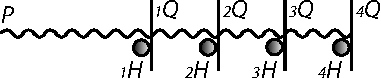
\includegraphics[width=0.42\textwidth]{gesamttex/edit_VIII,3/images/LH_35_10_08_010-011_d2.pdf}}%
%  \vspace*{0.5em}
%  \centerline{\hspace*{-55mm}\lbrack\textit{Fig.~2}\rbrack}%
%  \label{LH_35_10_08_011r_Fig.2}%
%%  \vspace*{1.5em}
%%
%  \vspace*{-8.0em}
%  \centerline{\hspace*{65mm}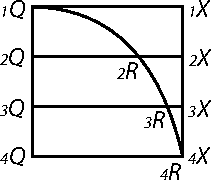
\includegraphics[width=0.24\textwidth]{gesamttex/edit_VIII,3/images/LH_35_10_08_010-011_d3.pdf}}%
%  \vspace*{0.0em}
%  \centerline{\hspace*{65mm}\lbrack\textit{Fig.~3}\rbrack}%
%  \label{LH_35_10_08_011r_Fig.3}%
%  \vspace*{1.0em}
%%
%%
\pstart%
A\edlabel{LH_35_10_08_010-011_ersterTeil-2}
consideratione\protect\index{Sachverzeichnis}{consideratio} compressionis\protect\index{Sachverzeichnis}{compressio aeris}
veniamus ad casum\protect\index{Sachverzeichnis}{casus} tensionis\protect\index{Sachverzeichnis}{tensio aeris}
ubi contrarium evenit,
cum enim potentia semper aestimanda sit ab effectu,\protect\index{Sachverzeichnis}{potentia ab effectu aestimanda}
patet
%
\edtext{\lbrack in compressione\rbrack}{\lemma{in}\Bfootnote{%
\hspace{-0,5mm}compressione
\textit{erg. Hrsg.}}}
%
eo majorem \makebox[1.0\textwidth][s]{esse effectum,\protect\index{Sachverzeichnis}{effectus}
quo minus est spatium\protect\index{Sachverzeichnis}{spatium compressionis}
in quod aer\protect\index{Sachverzeichnis}{aer inclusus} est inclusus;
contra in tensione,\protect\index{Sachverzeichnis}{tensio aeris}
\edtext{eo major}{%
\lemma{eo}\Bfootnote{%
\textit{(1)}~majus
\textit{(2)}~major%
~\textit{L}}}}
%
\pend
\newpage
\pstart 
\begin{minipage}[t]{0.5\textwidth}
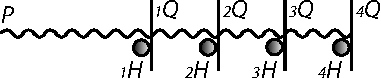
\includegraphics[width=0.9\textwidth]{gesamttex/edit_VIII,3/images/LH_35_10_08_010-011_d2.pdf}
\end{minipage}
\hspace{15mm}
\begin{minipage}[t]{0.5\textwidth}
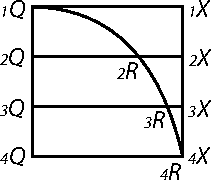
\includegraphics[width=0.49\textwidth]{gesamttex/edit_VIII,3/images/LH_35_10_08_010-011_d3.pdf}
\end{minipage}
\\
\\
\hspace*{31mm} [\textit{Fig.~2}]\label{LH_35_10_08_011r_Fig.2}\hspace*{57mm} [\textit{Fig.~3}] \label{LH_35_10_08_011r_Fig.3}
\pend
\vspace{1.5em}
\pstart
\noindent\setline{1}%
est potentia\protect\index{Sachverzeichnis}{potentia aeris tensi}
quo majus est spatium\protect\index{Sachverzeichnis}{spatium extensionis}
in quod corpus est vi extensum;%
\protect\index{Sachverzeichnis}{corpus vi extensum}
%
\edtext{quemadmodum alibi
\edtext{a me}{%
\lemma{a}\Bfootnote{%
\hspace{-0,5mm}me
\textit{erg.~L}}}
demonstratum est accuratius.}{%
\lemma{quemadmodum \lbrack...\rbrack\ accuratius}\Cfootnote{%
Siehe etwa in diesem Band N.~14\textsubscript{3}, S.~\refpassage{LH_35_09_16_020v_kolbenmodell-1}{LH_35_09_16_020v_kolbenmodell-2}, und N.~14\textsubscript{7}, S.~\refpassage{LH_35_09_16_002_Beweis-1}{LH_35_09_16_002_Beweis-2}.}}
%
\edtext{Sunt scilicet}{%
\lemma{Sunt}\Bfootnote{%
\textit{(1)}~ergo
\textit{(2)}~scilicet%
~\textit{L}}}
%
potentiae tendentes\protect\index{Sachverzeichnis}{potentia tendens}
ut spatia quae tensione\protect\index{Sachverzeichnis}{spatium extensionis}
\edtext{accessere.
Itaque corpus \textit{H} horizontaliter motum
atque incurrens\protect\index{Sachverzeichnis}{corpus incurrens}
in \textit{{\scriptsize1}Q} extremum chordae \textit{P{\scriptsize1}Q},\protect\index{Sachverzeichnis}{chorda tensa}
tendit\protect\index{Sachverzeichnis}{corpus tendens} ipsum}{%
\lemma{accessere}\Bfootnote{%
\textit{(1)}~, ergo celeritates quas corpus impetu suo
\textit{(a)}~tendens am
\textit{(b)}~chordam vel simile quid tendens amisit
\textit{(2)}~. Itaque corpus \textit{H}
\textit{(a)}~tendat chordam \textit{P{\scriptsize1}Q}
\textit{(b)}~horizontaliter motum \lbrack...\rbrack\ tendit ipsum%
~\textit{L}}}
%
ab \textit{{\scriptsize1}Q} in \textit{{\scriptsize2}Q},
inde in \textit{{\scriptsize3}Q},
denique in \textit{{\scriptsize4}Q},
ubi quiescat vi sua
\edtext{exhausta.\protect\index{Sachverzeichnis}{vis exhausta}
Cum ergo}{%
\lemma{exhausta.}\Bfootnote{%
\textit{(1)}~Itaque
\textit{(2)}~Cum ergo%
~\textit{L}}}
%
vires tensionis\protect\index{Sachverzeichnis}{vis tensionis}
seu vires tendentes\protect\index{Sachverzeichnis}{vis tendens}
sint ut rectae \textit{{\scriptsize1}Q{\scriptsize2}Q}, \textit{{\scriptsize1}Q{\scriptsize3}Q}, \textit{{\scriptsize1}Q{\scriptsize4}Q},
ergo vires\protect\index{Sachverzeichnis}{vis amissa}
quas corpus \textit{H} amisit\protect\index{Sachverzeichnis}{corpus tendens}
cum est in \textit{{\scriptsize2}Q}, \textit{{\scriptsize3}Q}, \textit{{\scriptsize4}Q}
sunt similiter ut \textit{{\scriptsize1}Q{\scriptsize2}Q}, \textit{{\scriptsize1}Q{\scriptsize3}Q},
\textit{{\scriptsize1}Q{\scriptsize4}Q}.
Celeritates autem quas amisit,\protect\index{Sachverzeichnis}{celeritas amissa}
sunt in subduplicata virium ratione,
\edtext{ergo celeritas\protect\index{Sachverzeichnis}{celeritas amissa}
\lbrack quam\rbrack\ corpus \textit{H} amisit\protect\index{Sachverzeichnis}{corpus tendens}
cum est in \textit{{\scriptsize2}H},
est ad celeritatem quam amisit\protect\index{Sachverzeichnis}{celeritas amissa}
cum est in \textit{{\scriptsize3}H},}{%
\lemma{ergo}\Bfootnote{%
\textit{(1)}~sunt celeritates
\textit{(2)}~celeritas
\textbar~quam \textit{erg.~Hrsg.}~%
\textbar\ corpus \textit{H}
\textit{(a)}~habet in \textit{{\scriptsize2}H} est ad celeritatem qu
\textit{(b)}~amisi
\textit{(c)}~amisit cum \lbrack...\rbrack\ est in \textit{{\scriptsize3}H},%
~\textit{L}}}
%
ut in subduplicata ratione
\textit{{\scriptsize1}Q{\scriptsize2}Q} ad \textit{{\scriptsize1}Q{\scriptsize3}Q}.
\edlabel{LH_35_10_08_011r_dritteMarg-1}%
\edtext{Hinc%
eodem modo argumentando
%
\edtext{ut supra,}{%
\lemma{ut supra}\Cfootnote{%
S.~\refpassage{LH_35_10_08_010r_utsupra_bguzbfiv-1}{LH_35_10_08_010r_utsupra_bguzbfiv-2};
\refpassage{LH_35_10_08_010v_utsupra_jzfgik-1}{LH_35_10_08_011r_utsupra_jzfgik-2}.}}%
\edlabel{LH_35_10_08_011r_dritteMarg-2}}{%
\lemma{\textit{Am Rand:}}\Afootnote{%
\Denarius\
(\protect\vphantom)%
Videtur hic ut supra\textsuperscript{\lbrack a\rbrack} subesse error.\protect\index{Sachverzeichnis}{error}
Vide finem schedae.\textsuperscript{\lbrack b\rbrack}\protect\index{Sachverzeichnis}{scheda}%
\protect\vphantom()% \\%
\vspace*{0.5em}%
\newline%
{\footnotesize%
\textsuperscript{\lbrack a\rbrack}~ut supra: S.~\refpassage{LH_35_10_08_010r_suurihuomaus-1}{LH_35_10_08_010r_suurihuomaus-2}; \refpassage{LH_35_10_08_010v_error2_dggwg-1}{LH_35_10_08_010v_error2_dggwg-2}
\quad%
\textsuperscript{\lbrack b\rbrack}~finem schedae: S.~\refpassage{LH_35_10_08_011v_finisschedae_avdf-1}{LH_35_10_08_011v_finisschedae_avdf-2}.}}}
%
si chorda\protect\index{Sachverzeichnis}{chorda dimissa} dimissa
et a \textit{{\scriptsize4}Q} ad \textit{{\scriptsize1}Q} rediens
corpus \textit{H} impellere\protect\index{Sachverzeichnis}{corpus impulsum}
%
\edtext{intelligatur,
erunt celeritates corporis \textit{H}\protect\index{Sachverzeichnis}{celeritas corporis impulsi}
adhuc acquirendae\protect\index{Sachverzeichnis}{celeritas acquirenda}
cum est in \textit{{\scriptsize3}H} vel \textit{{\scriptsize2}H},
seu}{%
\lemma{intelligatur,}\Bfootnote{%
\textit{(1)}~patet
\textit{(a)}~celeritatem
\textit{(b)}~celeritates residuas, quas
\textit{(2)}~et celeritas quam
\textit{(3)}~erunt celeritates \lbrack...\rbrack\ adhuc acquirendae
\textbar~cum est in \textit{{\scriptsize3}H} vel \textit{{\scriptsize2}H} \textit{erg.}~%
\textbar~, seu%
~\textit{L}}}
%
differentiae inter ibi quaesitas\protect\index{Sachverzeichnis}{celeritas quaesita}
et summam
\pend
\newpage
\pstart
\noindent quam habebit in \textit{{\scriptsize1}H},
in subduplicata ratione spatiorum adhuc\protect\index{Sachverzeichnis}{spatium percurrendum}
\edtext{percurrendorum \textit{{\scriptsize1}Q{\scriptsize3}Q}, \textit{{\scriptsize1}Q{\scriptsize2}Q}.}{%
\lemma{percurrendorum}\Bfootnote{%
\textit{(1)}~seu celeritas quam corpus \textit{H} acquisit\lbrack\textit{!}\rbrack\ in \textit{{\scriptsize3}H}
\textit{(2)}~\textit{{\scriptsize1}Q{\scriptsize3}Q}, \textit{{\scriptsize1}Q{\scriptsize2}Q}.%
~\textit{L}}}
%
Unde aestimari potest vis arcus tensi.%
\protect\index{Sachverzeichnis}{vis arcus}\protect\index{Sachverzeichnis}{vis aestimanda}\protect\index{Sachverzeichnis}{arcus tensus}
\pend%
% \newpage%
%
%
\pstart%
\edtext{Videamus jam}{%
\lemma{Vide-}\Bfootnote{%
amus \textit{(1)}~et
\textit{(2)}~jam%
~\textit{L}}}
%
hinc quae
\edtext{sit inter tempora et spatia relatio,%
\protect\index{Sachverzeichnis}{relatio temporis et spatii}}{%
\lemma{sit}\Bfootnote{%
\textit{(1)}~ratio
\textit{(2)}~inter tempora et spatia relatio,%
~\textit{L}}}
%
seu celeritates\protect\index{Sachverzeichnis}{celeritas restitutionis}
\edtext{adhuc deficientes}{%
\lemma{adhuc}\Bfootnote{%
\textit{(1)}~acquirendae
\textit{(2)}~deficientes%
~\textit{L}}}
%
cum corpus \textit{H}\protect\index{Sachverzeichnis}{corpus projiciendum}
est in \textit{{\scriptsize3}Q} vel \textit{{\scriptsize2}Q}
si repraesententur per rectas
\textit{{\scriptsize3}Q{\scriptsize3}R},
%
\edtext{\lbrack\textit{{\scriptsize2}Q{\scriptsize2}R}\rbrack,}{%
\lemma{\textit{{\scriptsize4}Q{\scriptsize4}R}}\Bfootnote{%
\textit{L~ändert Hrsg.}}}
%
erunt ut ordinatae parabolae\protect\index{Sachverzeichnis}{parabola}
cujus vertex \textit{{\scriptsize1}Q},
Axis \textit{{\scriptsize1}Q{\scriptsize4}Q},
basis \textit{{\scriptsize4}Q{\scriptsize4}R} axi,
si placet altitudini, aequalis,
nam is pro arbitrio\protect\index{Sachverzeichnis}{arbitrium} sumi potest.
Quod si
\edtext{ergo parabolico Trilineo\protect\index{Sachverzeichnis}{trilineum parabolicum}
\lbrack convexo\rbrack\
\textit{{\scriptsize1}Q{\scriptsize4}Q{\scriptsize4}R{\scriptsize1}Q}}{%
\lemma{ergo}\Bfootnote{\hspace{-0,5mm}%
\textbar~semi \textit{gestr.}~%
\textbar\ parabolico Trilineo
\textbar~concavo \textit{ändert Hrsg.}~%
\textbar\ \textit{{\scriptsize1}Q{\scriptsize4}Q{\scriptsize4}R{\scriptsize1}Q}%
~\textit{L}}}
%
circumscribatur
\edtext{quadratum\protect\index{Sachverzeichnis}{quadratum}
\lbrack\textit{{\scriptsize1}Q{\scriptsize4}Q{\scriptsize4}R{\scriptsize1}X}\rbrack\
et sit latus}{%
\lemma{quadratum}\Bfootnote{%
\textit{(1)}~\textit{{\scriptsize1}Q{\scriptsize4}Q{\scriptsize4}R{\scriptsize4}S}
\textit{(2)}~\textbar~\textit{{\scriptsize1}Q{\scriptsize4}Q{\scriptsize4}R{\scriptsize4}X} \textit{ändert Hrsg.}~%
\textbar\ et
\textit{(a)}~ducantur ipsae in
\textit{(b)}~sit latus%
~\textit{L}}}
%
\textit{XX} oppositum lateri \textit{QQ},
erunt ipsae \textit{RX} celeritates\protect\index{Sachverzeichnis}{celeritas restitutionis}
a corpore projiciendo\protect\index{Sachverzeichnis}{corpus projiciendum}
quaesitae.
Porro generaliter scimus
Temporibus\protect\index{Sachverzeichnis}{tempus restitutionis} existentibus \textit{t},
locis seu spatiis \textit{l},\protect\index{Sachverzeichnis}{spatium restitutionis}
celeritatibus\protect\index{Sachverzeichnis}{celeritas restitutionis}
quaesitis \textit{c},\protect\index{Sachverzeichnis}{celeritas quaesita}
fore \textit{l} aequ.
\edtext{$\displaystyle\!\!\int\!\!\overline{\frac{c}{a}dt}.$}{%
\lemma{$\displaystyle\!\!\int\!\!\overline{\frac{c}{a}dt}$}\Cfootnote{%
\textit{a} ist offenbar die Seite \textit{{\scriptsize{1}}Q{\scriptsize{1}}X} des Quadrats \textit{{\scriptsize{1}}Q{\scriptsize{4}}Q{\scriptsize{4}}R{\scriptsize{1}}X} bzw. die maximale Geschwindigkeit, die der Körper \textit{H} in \textit{{\scriptsize{1}}Q} zurückgewinnt.}}
%
Ergo \textit{dla} aequ. \textit{cdt} ergo \textit{t} aequ. $\displaystyle\!\!\int\!\!\overline{adl:c}.$
Sunt autem hoc
\edlabel{LH_35_10_08_010-011_e011v1}loco%
\edtext{}{{\xxref{LH_35_10_08_010-011_e011v1}{LH_35_10_08_010-011_e011v2}}%
{\lemma{loco}\Bfootnote{\hspace{-0,5mm}
\textit{(1)}~\textit{RX} seu \textit{c} aeq. $\sqrt{\!ac}\,a$ \lbrack11~v\textsuperscript{o}\rbrack\
\textit{(2)}~\textbar~\textit{R{\scriptsize3}X} \textit{ändert Hrsg.}~%
\textbar\ seu \textit{c} aequ. $QX - {\scriptstyle\textit{3}}Q{\scriptstyle\textit{3}}R$%
~\textit{L}}}}
%
\lbrack11~v\textsuperscript{o}\rbrack\ %%%% Blatt 11v
%
\lbrack\textit{{\scriptsize3}R{\scriptsize3}X}\rbrack\ seu \textit{c} aequ. $QX-{\scriptstyle\textit{3}}Q{\scriptstyle\textit{3}}R$\edlabel{LH_35_10_08_010-011_e011v2}
%
seu $\displaystyle QX-\sqrt{QX\cdot{\scriptstyle\textit{1}}Q{\scriptstyle\textit{3}}Q}$ seu \textit{c} aequ. $a-\sqrt{\!al}$ ergo fiet: \textit{t} aequ. $\displaystyle\!\!\int\!\!\overline{adl:\overline{a-\sqrt{\!al}}}$ cujus ineunda est
\edtext{summa: $\displaystyle a-\sqrt{\protect\vphantom{\protect\mathstrut al}}\!al$ aequ. \textit{c}}{%
\lemma{summa:}\Bfootnote{%
\textit{(1)}~Sit:
\textit{(2)}~$\displaystyle a-\sqrt{\protect\vphantom{\protect\mathstrut al}}\!al$ aequ. \textit{c}%
~\textit{L}}}
%
et $cc-2ca+aa$ aequ. \textit{al}.
Ergo \textit{adl} aequ. $2cdc-2adc$ et fiet: \textit{t} aequ. $\displaystyle\!\!\int\!\!\overline{2\xout{c}dc:\xout{c}}-\!\!\int\!\!\overline{2adc:c}$ seu fiet: \textit{t} aequ. $\displaystyle2c-2a\!\!\int\!\!\overline{dc:c}$ seu $2c-2a$ log\,\textit{c}. aequ. \textit{t}.
Erunt ergo tempora\protect\index{Sachverzeichnis}{tempora restitutionis}
proportionalia quantitatibus compositis ex differentiis
inter celeritates,\protect\index{Sachverzeichnis}{celeritas restitutionis}
et celeritatum logarithmos Hyperbolicos\protect\index{Sachverzeichnis}{logarithmus hyperbolicus}
Unitatem primariam habentes maximam celeritatem.\protect\index{Sachverzeichnis}{celeritas maxima}
Re autem ad spatia\protect\index{Sachverzeichnis}{spatium restitutionis}
seu loca sive \textit{l} revocata,
% \rule[0pt]{0mm}{10pt}
erunt
\edtext{\textit{t} aequ. $\displaystyle a-\sqrt{\protect\vphantom{\protect\mathstrut al}}\!al-2a\!\!\int\!\!\overline{-\frac{1}{2}\frac{dl}{\displaystyle\sqrt{\protect\vphantom{\protect\mathstrut al}}\!al}:a-\sqrt{\protect\vphantom{\protect\mathstrut al}}\!al}$ seu \textit{t} aequ.
$\displaystyle a-\sqrt{\protect\vphantom{\protect\mathstrut al}}\!al-a
\!\!\int\!\!\overline{dl:\overline{\sqrt{\!al}-l}}.$}{%
\lemma{\textit{t} aequ. \lbrack...\rbrack\ $a-\sqrt{\protect\vphantom{\displaystyle\protect\mathstrut al}}\displaystyle\!al-a \!\!\int\!\!\overline{dl:\overline{\sqrt{\!al}-l}}\,$}\Cfootnote{%
Die Gleichung heißt eigentlich:
$\displaystyle t = 2 (a - \sqrt{al}) + a \!\!\int\!\!\frac{dl}{a (\sqrt{al} - l)}.$%
% Der umgeformte Integrand lautet eigentlich: $\displaystyle dl:a(\sqrt{\!al}-1)$
}}
%
\edtext{Sed de signis\protect\index{Sachverzeichnis}{signum} accuratius constituendum.}{%
\lemma{Sed}\Bfootnote{%
\hspace{-0,5mm}de signis accuratius constituendum.
\textit{erg.~L}}}
\pend%
%
\newpage
\count\Bfootins=900
\count\Afootins=1200
\count\Cfootins=900
\pstart%
Hinc
\edtext{patet
variantibus spatiis \textit{l} tempora quoque \textit{t} variari,%
\protect\index{Sachverzeichnis}{tempus restitutionis}\protect\index{Sachverzeichnis}{spatium restitutionis}
adeoque ad restitutionem\protect\index{Sachverzeichnis}{restitutio corporis tensi} corporis tensi,
corporis tendentis rejectione\protect\index{Sachverzeichnis}{rejectio corporis tendentis} oneratam,
alio atque alio tempore opus fore,
prout magis minusve ab eo tensum est.}{%
\lemma{patet}\Bfootnote{%
\textit{(1)}~variantibus
\textit{(2)}~crescentibus
\textit{(3)}~variantibus spatiis
\textbar~\textit{l} \textit{erg.}~\textbar~%
\textit{(a)}~variari
\textit{(b)}~tempora quoque \textit{t}
\textit{(aa)}~crescere
\textit{(bb)}~variari,
\textit{(aaa)}~seu
\textit{(bbb)}~seu majore tempore fore
\textit{(ccc)}~adeoque
\textbar~opus \textit{streicht Hrsg.}~%
\textbar\ ad restitutionem \lbrack...\rbrack\ corporis tendentis % corporis tensi,
\textit{(aaaa)}~restituti
\textit{(bbbb)}~rejectione oneratam,
\textit{(aaaaa)}~prout id majore
\textit{(bbbbb)}~alio atque \lbrack...\rbrack\ tensum est.%
~\textit{L}}}
%
% \pend%
%
%
% \pstart%
Sed tamen
%
\edtext{alias si bene memini demonstravi}{%
\lemma{alias \lbrack...\rbrack\ demonstravi}\Cfootnote{%
Vermutlich Anspielung auf N.~8\textsubscript{5} (S.~\refpassage{LH_35_09_15_015v_isochron-1}{LH_35_09_15_015v_isochron-2}) und N.~9 (S.~\refpassage{LH_35_09_15_003r_aequdiut-1}{LH_35_09_15_003v_aequdiut-2}).
In diesen Entwürfen hatte Leibniz im Dezember 1680 den Isochronismus der \textit{restitutio omnimoda} einer schwingenden Saite geometrisch nachzuweisen versucht.
Die Fomulierung \textit{si bene memini} deutet jedenfalls auf einen bereits einige Jahre alten Beweisgang hin.
Dem Isochronismus der Schwingungen widmete sich Leibniz auch in späteren Entwürfen
wie N.~\ref{RK60301} %??A45 
und N.~\ref{RK60353} %??A46
(1690 bis 1695).
}}
%
corpus tensum\protect\index{Sachverzeichnis}{corpus tensum}
si inter restituendum%
\protect\index{Sachverzeichnis}{restitutio corporis tensi}
nullo modo oneratum intelligatur,
seu si abstrahatur animus\protect\index{Sachverzeichnis}{animus}
a pondere naturaliter ei adhaerente,%
\protect\index{Sachverzeichnis}{pondus corporis tensi}
sese eodem semper tempore restituturum.%
\protect\index{Sachverzeichnis}{restitutio isochrona}
\pend%
%
%
\pstart%
Caeterum video tamen hic magnam esse difficultatem.\protect\index{Sachverzeichnis}{difficultas}
Nam cum semper mole\protect\index{Sachverzeichnis}{moles corporis tensi}
suae materiae\protect\index{Sachverzeichnis}{materia corporis tensi} oneratum sit,
videtur perinde esse ac si eam rejicere conaretur.
Itaque perinde est ac si
\edtext{fingatur ab ejus incursu}{%
\lemma{fingatur}\Bfootnote{%
\textit{(1)}~ab ea ini
\textit{(2)}~ab ejus incursu%
~\textit{L}}}
%
fuisse tensum.
Et licet exiguum
\edtext{admodum ponatur}{%
\lemma{admodum}\Bfootnote{%
\textit{(1)}~videatur
\textit{(2)}~ponatur%
~\textit{L}}}
%
pondus,
tamen res eodem redit,
quia tanto majore celeritate fingi debet tetendisse.\protect\index{Sachverzeichnis}{celeritas corporis tensi}
Ergo tanto majorem celeritatem ei communicabit.\protect\index{Sachverzeichnis}{celeritas communicata}
\pend%
%
%
\pstart%
Itaque\edlabel{LH_35_10_08_011v_finisschedae_avdf-1} re recte considerata,
in eo a me peccatum videtur
quod supposui Elastrum se restituens\protect\index{Sachverzeichnis}{Elastrum se restituens}
vim eodem modo reddere\protect\index{Sachverzeichnis}{vis reddita}
corpori\protect\index{Sachverzeichnis}{corpus tendens}
cujus impulsu tensum fuerat,%
\protect\index{Sachverzeichnis}{impulsus corporis tendentis}\protect\index{Sachverzeichnis}{elastrum tensum}
quo eam ab eo accepit.
Ita enim
\edtext{sequetur arcum\protect\index{Sachverzeichnis}{arcus tensus}
(\protect\vphantom)%
si is illapsu sagittae\protect\index{Sachverzeichnis}{sagitta} tensus ponatur%
\protect\vphantom()
quolibet momento impulsus totam vim\protect\index{Sachverzeichnis}{vis impulsus}
quam Elastrum\protect\index{Sachverzeichnis}{Elastrum se restituens} perdidit,
accipere,}{%
\lemma{sequetur}\Bfootnote{%
\textit{(1)}~ipsum totum impetum conceptum
\textit{(2)}~arcum (\protect\vphantom)si \lbrack...\rbrack\ perdidit, accipere,%
~\textit{L}}}
%
cum tamen ipsa materia arcus\protect\index{Sachverzeichnis}{materia arcus}
etiam plurimum de impetu concepto\protect\index{Sachverzeichnis}{impetus conceptus} retineat;
eoque ipso ad celeritatem mox secuturae residuae detensionis seu restitutionis augendam
%
\edtext{contribuat.
In quo interest}{%
\lemma{contribuat.}\Bfootnote{%
\textit{(1)}~Itaque quo mi
\textit{(2)}~In quo interest%
~\textit{L}}}
%
inter sagittam\protect\index{Sachverzeichnis}{sagitta}
et onus\protect\index{Sachverzeichnis}{onus elastri} naturaliter adhaerens ipsi elastro,
seu materiam\protect\index{Sachverzeichnis}{materia chordae}
%
\edtext{chordae,\protect\index{Sachverzeichnis}{chorda arcus}
hoc onus\protect\index{Sachverzeichnis}{onus elastri} enim}{%
\lemma{chordae,}\Bfootnote{%
\textit{(1)}~ea
\textit{(2)}~hoc
\textbar~onus \textit{erg.}~%
\textbar\ enim%
~\textit{L}}}
%
impetu concepto\protect\index{Sachverzeichnis}{impetus conceptus}
\edtext{\lbrack quem\rbrack}{%
\lemma{quam}\Bfootnote{%
\textit{L~ändert Hrsg.}}}
%
elastrum perdidit,\protect\index{Sachverzeichnis}{elastrum se restituens}
restitutionem\protect\index{Sachverzeichnis}{restitutio elastri} tamen adhuc promovet.
At sagitta\protect\index{Sachverzeichnis}{sagitta} hoc non
%
\edtext{facit,
nisi arcui\protect\index{Sachverzeichnis}{arcus tensus} alligata ponatur,
et impetum acceperit majorem eundi,\protect\index{Sachverzeichnis}{impetus eundi}}{%
\lemma{facit,}\Bfootnote{%
\textit{(1)}~impetus enim ab ea conceptus, etiam si arcui alligata
\textit{(2)}~nisi arcui \lbrack...\rbrack\ et impetum
\textit{(a)}~habeat ma
\textit{(b)}~acceperit majorem eundi,%
~\textit{L}}}
%
quam ipsae
\edtext{partes arcus\protect\index{Sachverzeichnis}{arcus tensus}
vel chordae\protect\index{Sachverzeichnis}{chorda arcus}
quibus alligata}{%
\lemma{partes}\Bfootnote{%
\textit{(1)}~chordae quibus alli
\textit{(2)}~arcus vel chordae quibus alligata%
~\textit{L}}}
%
est;
nam si minorem, ut solet, potius retardat.
Absolute tamen loquendo semper tardat,
quicquid arcum\protect\index{Sachverzeichnis}{arcus tensus} onerat magis.
At materia ipsa\protect\index{Sachverzeichnis}{materia arcus}
ex qua arcus componitur
tanto minus onerat,
quanto purius elastica\protect\index{Sachverzeichnis}{materia elastica} est.\edlabel{LH_35_10_08_011v_finisschedae_avdf-2}
\pend 
\count\Bfootins=1200
\count\Afootins=1200
\count\Cfootins=1200
%
%
%%%%    Ende des <stücks auf Blatt 11v